%!TEX program = xelatex
\documentclass[a4paper,11pt]{article}
\usepackage{kotex}
\usepackage{amsmath,amssymb}
\usepackage{geometry}
\usepackage{multicol}
\usepackage{array}
\usepackage{enumitem}
\usepackage{tikz}
\usepackage{xcolor}
\usepackage{mdframed}

\geometry{top=15mm, bottom=15mm, left=15mm, right=15mm}

\setmainfont{NanumMyeongjo}
\setsansfont{NanumGothic}

\setlength{\columnseprule}{0.4pt}
\setlength{\columnsep}{8mm}

\newcommand{\choicenum}[1]{\textcircled{\small #1}}
\newcommand{\scorebox}[1]{\textbf{(#1점)}}
\newcommand{\qbox}[1]{%
  \begin{mdframed}[linewidth=0.8pt,innerleftmargin=6pt,innerrightmargin=6pt,innertopmargin=4pt,innerbottommargin=4pt]
  #1
  \end{mdframed}
}

\pagestyle{empty}

\begin{document}

%--- 헤더 ---
\begin{center}
{\large \textbf{3학년 1학기 중간고사 \quad 수학 \quad [C형]}}\\[2pt]
{\normalsize 선택형 1번\,--\,16번 \;/\; 서술형 1번\,--\,8번 \quad 총 4쪽}
\end{center}
\vspace{1mm}
\hrule height 1pt
\vspace{3mm}

\begin{multicols}{2}

%===========================================================
%  선택형
%===========================================================

\noindent\textbf{1.} $\sqrt{81}$의 제곱근은? \scorebox{3}

\begin{enumerate}[label=\protect\choicenum{\arabic*},leftmargin=*,itemsep=0pt]
  \item $9$
  \item $-9$
  \item $\pm\,3$
  \item $\pm\,9$
  \item $81$
\end{enumerate}

\vspace{3mm}

\noindent\textbf{2.} 실수의 대소관계로 옳은 것은? \scorebox{3}

\begin{enumerate}[label=\protect\choicenum{\arabic*},leftmargin=*,itemsep=0pt]
  \item $\sqrt{17} < 4$
  \item $\sqrt{7} > 3$
  \item $-\sqrt{6} > -2$
  \item $-\sqrt{35} < -6$
  \item $\dfrac{\sqrt{6}}{3} > \dfrac{\sqrt{10}}{3}$
\end{enumerate}

\vspace{3mm}

\noindent\textbf{3.} 다음을 계산하면? \scorebox{3}

\qbox{$\sqrt{18} \div \sqrt{3} \times 4\sqrt{6}$}

\begin{enumerate}[label=\protect\choicenum{\arabic*},leftmargin=*,itemsep=0pt]
  \item $4\sqrt{6}$
  \item $12\sqrt{6}$
  \item $24\sqrt{6}$
  \item $36\sqrt{6}$
  \item $48\sqrt{6}$
\end{enumerate}

\vspace{3mm}

\noindent\textbf{4.} 다음 식을 전개하면? \scorebox{3}

\qbox{$(5x+y)(5x-y)$}

\begin{enumerate}[label=\protect\choicenum{\arabic*},leftmargin=*,itemsep=0pt]
  \item $5x^{2}-y^{2}$
  \item $25x^{2}-y^{2}$
  \item $25x^{2}+y^{2}$
  \item $25x^{2}+10xy-y^{2}$
  \item $25x^{2}-10xy+y^{2}$
\end{enumerate}

\vspace{3mm}

\noindent\textbf{5.} 다음 식이 완전제곱식이 되도록\\
\quad $\square$ 안에 알맞은 수를 고르면? \scorebox{3}

\qbox{$16x^{2}-40x+\square$}

\begin{enumerate}[label=\protect\choicenum{\arabic*},leftmargin=*,itemsep=0pt]
  \item $4$
  \item $16$
  \item $20$
  \item $25$
  \item $100$
\end{enumerate}

\vspace{3mm}

\noindent\textbf{6.} 다음 이차방정식을 풀면? \scorebox{3}

\qbox{$x^{2}-7x=0$}

\begin{enumerate}[label=\protect\choicenum{\arabic*},leftmargin=*,itemsep=0pt]
  \item $x=7$
  \item $x=0$ 또는 $x=7$
  \item $x=0$ 또는 $x=-7$
  \item $x=-7$ 또는 $x=7$
  \item $x=0$
\end{enumerate}

\vspace{3mm}

\noindent\textbf{7.} 무리수만으로 짝지어진 것을 고르면? \scorebox{4}

\begin{enumerate}[label=\protect\choicenum{\arabic*},leftmargin=*,itemsep=0pt]
  \item $\sqrt{1},\,\sqrt{4},\,\sqrt{9}$
  \item $\sqrt{\dfrac{1}{4}},\,\sqrt{0.04},\,\sqrt{3}$
  \item $1.5,\,\dfrac{4}{9},\,\sqrt{16}$
  \item $\sqrt{5},\,\sqrt{7},\,-\sqrt{0.49}$
  \item $\sqrt{0.64},\,-\sqrt{(-4)^{2}},\,\sqrt{36}+1$
\end{enumerate}

\vspace{3mm}

\noindent\textbf{8.} $0<x<1$일 때, 다음 중 가장 작은 것은? \scorebox{4}

\begin{enumerate}[label=\protect\choicenum{\arabic*},leftmargin=*,itemsep=0pt]
  \item $\sqrt{x}$
  \item $x$
  \item $x^{2}$
  \item $\dfrac{1}{x}$
  \item $3x$
\end{enumerate}

\vspace{3mm}

\noindent\textbf{9.} 다음을 계산하면? \scorebox{4}

\qbox{$2\sqrt{45}-\sqrt{20}+3\sqrt{5}$}

\begin{enumerate}[label=\protect\choicenum{\arabic*},leftmargin=*,itemsep=0pt]
  \item $5\sqrt{5}$
  \item $7\sqrt{5}$
  \item $9\sqrt{5}$
  \item $11\sqrt{5}$
  \item $13\sqrt{5}$
\end{enumerate}

\vspace{3mm}

\noindent\textbf{10.} $\sqrt{27}\!\left(\dfrac{\sqrt{3}}{3}-1\right)+\dfrac{a}{\sqrt{3}}\!\left(\sqrt{75}-3\right)$이\\
유리수일 때, 유리수 $a$의 값을 구하면? \scorebox{4}

\begin{enumerate}[label=\protect\choicenum{\arabic*},leftmargin=*,itemsep=0pt]
  \item $\dfrac{3}{5}$
  \item $1$
  \item $\dfrac{3}{4}$
  \item $\dfrac{5}{4}$
  \item $-1$
\end{enumerate}

\vspace{3mm}

\noindent\textbf{11.} 식을 전개할 때, $x$의 계수가 다른 하나는? \scorebox{4}

\begin{enumerate}[label=\protect\choicenum{\arabic*},leftmargin=*,itemsep=0pt]
  \item $(x+1)(x-8)$
  \item $(x+7)(-x+2)$
  \item $(x+4)(2x-3)$
  \item $(4x+1)(2x-3)$
  \item $(3x+1)(3x-5)$
\end{enumerate}

\vspace{3mm}

\noindent\textbf{12.} 다음 식을 전개하면? \scorebox{4}

\qbox{$(2x+y)^{2}-25\!\left(\dfrac{1}{5}x+y\right)^{2}$}

\begin{enumerate}[label=\protect\choicenum{\arabic*},leftmargin=*,itemsep=0pt]
  \item $-6xy-21y^{2}$
  \item $6xy+21y^{2}$
  \item $3x^{2}-6xy-3y^{2}$
  \item $3x^{2}+6xy-21y^{2}$
  \item $3x^{2}-y^{2}$
\end{enumerate}

\vspace{3mm}

\noindent\textbf{13.} 다음 두 다항식을 인수분해 할 때, 공통으로 들어 있는 인수는? \scorebox{4}

\qbox{$-(x-5)+4x(x-5),\quad 8x^{2}+2x-3$}

\begin{enumerate}[label=\protect\choicenum{\arabic*},leftmargin=*,itemsep=0pt]
  \item $x-5$
  \item $4x-1$
  \item $4x+1$
  \item $2x-1$
  \item $2x+3$
\end{enumerate}

\vspace{3mm}

\noindent\textbf{14.} 다음 그림과 같은 직사각형의 빗금친 부분의 넓이를 구하면? \scorebox{4}

\begin{center}
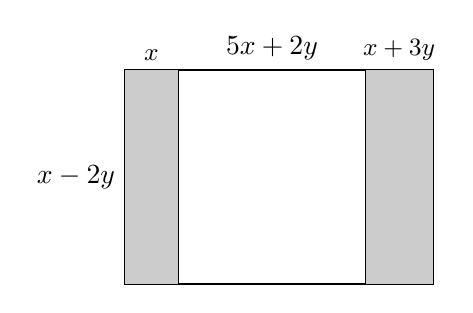
\begin{tikzpicture}[scale=0.85]
  \draw[thick] (0,0) rectangle (4.6,3.2);
  \draw[thick] (0.8,0) rectangle (3.6,3.2);
  \fill[gray!40] (0,0) rectangle (0.8,3.2);
  \fill[gray!40] (3.6,0) rectangle (4.6,3.2);
  \node[above] at (2.2,3.2) {$5x+2y$};
  \node[above] at (0.4,3.2) {\small $x$};
  \node[above] at (4.1,3.2) {\small $x+3y$};
  \node[left] at (0,1.6) {$x-2y$};
\end{tikzpicture}
\end{center}

\begin{enumerate}[label=\protect\choicenum{\arabic*},leftmargin=*,itemsep=0pt]
  \item $2x^{2}-4xy+6xy-12y^{2}$
  \item $2x^{2}+2xy-6y^{2}$
  \item $3x^{2}-8xy+3y^{2}$
  \item $3x^{2}+2xy-6y^{2}$
  \item $3x^{2}+4xy-12y^{2}$
\end{enumerate}

\vspace{3mm}

\noindent\textbf{15.} $\dfrac{1}{3}<x<5$일 때, 다음 식을 간단히 하면? \scorebox{5}

\qbox{$\sqrt{9x^{2}-6x+1}-\sqrt{x^{2}-10x+25}$}

\begin{enumerate}[label=\protect\choicenum{\arabic*},leftmargin=*,itemsep=0pt]
  \item $-3x+6$
  \item $2x-6$
  \item $4x-4$
  \item $2x+4$
  \item $-2x+4$
\end{enumerate}

\vspace{3mm}

\noindent\textbf{16.} 두 자연수 $a,\,b$에 대하여 다항식 $6x^{2}+7x+k$가\\
$(2x+a)(3x+b)$로 인수분해 되도록 하는 실수 $k$의\\
최댓값은? \scorebox{5}

\begin{enumerate}[label=\protect\choicenum{\arabic*},leftmargin=*,itemsep=0pt]
  \item $1$
  \item $2$
  \item $3$
  \item $4$
  \item $6$
\end{enumerate}

\end{multicols}

\newpage

%===========================================================
%  서술형
%===========================================================
\begin{center}
{\large \textbf{서술형 \quad [C형]}}
\end{center}
\noindent{\small ※ 서술형 문항은 \textbf{서술형 답지}에 풀이과정과 답을 쓰고 제출해야 합니다.}
\vspace{4mm}
\hrule
\vspace{4mm}

\begin{enumerate}[leftmargin=*,itemsep=10mm]

\item[\textbf{서술형 1.}] $\dfrac{2\sqrt{6}-3}{\sqrt{6}}$의 분모를 유리화하여라. \scorebox{4}

\vspace{30mm}

\item[\textbf{서술형 2.}] 다음 식을 전개하여라. \scorebox{4}

\qbox{$(2x-3)^{2}+5x(x-1)$}

\vspace{35mm}

\item[\textbf{서술형 3.}] 다음 이차방정식을 인수분해를 이용하여 풀어라. \scorebox{5}

\qbox{$6x^{2}-x-12=0$}

\vspace{35mm}

\item[\textbf{서술형 4.}] $\sqrt{\dfrac{1440}{x}}$이 자연수가 되도록 하는 자연수 $x$의 값을 모두 구하여라. \scorebox{5}

\vspace{35mm}

\item[\textbf{서술형 5.}] 이차식 $ax^{2}+3x-10$, $x^{2}+bx-4$의\\
공통인수가 $x+2$일 때, $a-b$의 값을 구하여라. \scorebox{5}

\vspace{35mm}

\item[\textbf{서술형 6.}] $2^{2}-4^{2}+6^{2}-8^{2}+10^{2}-12^{2}$을\\
인수분해를 이용하여 계산하여라. \scorebox{5}

\vspace{35mm}

\item[\textbf{서술형 7.}] 다음 두 부등식을 모두 만족시키는 자연수 $x$의\\
값을 모두 더하면? \scorebox{6}

\qbox{%
\begin{tabular}{l}
① $\sqrt{12} < 2\sqrt{x} < \sqrt{40}$ \\[4pt]
② $-5 < -\sqrt{3x} < -3$
\end{tabular}
}

\vspace{40mm}

\item[\textbf{서술형 8.}] 사다리꼴 $ABCD$의 넓이를 구하고, 이것이\\
직사각형 $PQRS$의 넓이의 몇 배인지 구하여라. \scorebox{6}

\begin{center}
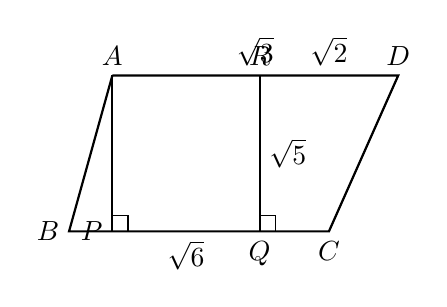
\begin{tikzpicture}[scale=1.1]
  \coordinate (A) at (0.5,1.8);
  \coordinate (D) at (3.8,1.8);
  \coordinate (B) at (0,0);
  \coordinate (C) at (3.0,0);
  \coordinate (P) at (0.5,0);
  \coordinate (Q) at (2.2,0);
  \coordinate (R) at (2.2,1.8);
  \draw[thick] (A)--(D)--(C)--(B)--(A);
  \draw[thick] (P)--(A);
  \draw[thick] (Q)--(R);
  \draw (P) rectangle ++(0.18,0.18);
  \draw (Q) rectangle ++(0.18,0.18);
  \node[above] at (A) {$A$};
  \node[above] at (D) {$D$};
  \node[left] at (B) {$B$};
  \node[below] at (C) {$C$};
  \node[left] at (P) {$P$};
  \node[below] at (Q) {$Q$};
  \node[above] at (R) {$R$};
  \node[below] at (1.35,0) {$\sqrt{6}$};
  \node[right] at (2.2,0.9) {$\sqrt{5}$};
  \node[above] at (2.15,1.8) {$\sqrt{3}$};
  \node[above] at (3.0,1.8) {$\sqrt{2}$};
\end{tikzpicture}
\end{center}

\end{enumerate}

\end{document}
